\chapter{Evaluation}
  \section{Data collection method and data collected}
    Table~\ref{tab:data-collected} details the amount of evaluation data collected.
    
    The data was collected with the smartwatch worn on the left wrist and the phone loose in the right hand trouser pocket.
    % Statistics about data gathered: how many records, total length etc.
    \begin{table}
      \centering
        \begin{tabular}{lrrr}
\toprule
      Activity &  Counts &  Proportion &  Time recorded (minutes) \\
\midrule
       Walking &     354 &      19.49\% &                       59 \\
    Gymcycling &     291 &      16.02\% &                       48 \\
       Cycling &     286 &      15.75\% &                       48 \\
      Fussball &     173 &       9.53\% &                       29 \\
        Eating &     172 &       9.47\% &                       29 \\
   Computeruse &     165 &       9.09\% &                       28 \\
      Standing &      92 &       5.07\% &                       15 \\
        Stairs &      76 &       4.19\% &                       13 \\
       Running &      62 &       3.41\% &                       10 \\
       Gallery &      59 &       3.25\% &                       10 \\
 Teethbrushing &      49 &       2.70\% &                        8 \\
      Climbing &      37 &       2.04\% &                        6 \\
         Total &    1816 &     100.00\% &                      303 \\
\bottomrule
\end{tabular}

      \caption{A summary of data collected.}
      \label{tab:data-collected}
    \end{table}
  \section{Evaluation process}
    Once the data was gathered, it was processed and features were extracted according to Section~\ref{sec:data-processing}.
    
    The data set was then split into training set and a testing set. This was done with a stratified shuffling splitter. This means that the proportional distribution of true labels in the testing set follows that of the training set. Whether an instance is placed in the training set or the testing set is chosen at random.
    
    The split was performed 10 times, with elements chosen at random each time. The splitter does not guarantee that the same split will not be made on subsequent splits, but such an event is unlikely given the size of the dataset.
    
    The data set was split in the ratio 50:50 training:testing.
    
    Once the data had been split, the labels were stripped from the testing data and set aside. Then, three separate instances of each of the four classifiers was trained on the training set. Each of the three instances only had access to features extracted from the phone accelerometer data, features extracted from the watch accelerometer data and both the phone-extracted and the watch-extracted features respectively.
    
    Each of the three instances were then tested on the test set and their evaluation metrics --- confusion matrix and $\mathrm{F}_1$ measure --- were calculated by comparing the true labels to the classified labels.
  \section{Evaluation metrics}
    Two primary methods of evaluation are used in this project: $\mathrm{F}_1$ measure and the confusion matrix.
    This section details these methods of evaluation. These metrics are discussed in Sokolova \emph{et al.}\cite{sokolova2009systematic}
    \subsection{F1 measure}
      In order to define the $\mathrm{F}_1$ measure, it is necessary to first define precision and recall. In a 
      \begin{description}
        \item[Precision], defined as $\frac{\text{True positives}}{\text{True postives} + \text{False positives}}$, is the proportion of instances of a particular label in which the classifier's labels agree with the true labels.
        \item[Recall], defined as $\frac{\text{True positives}}{\text{True postives} + \text{False negatives}}$, is the proportion of all the instances with a particular label which are labelled as such. 
      \end{description}
      
      The $\mathrm{F}_1$ measure is then defined as the harmonic mean of precision and recall:
      
      $$\mathrm{F}_1 = 2 \cdot \frac{\mathrm{precision} \cdot \mathrm{recall}}{\mathrm{precision} + \mathrm{recall}}$$
      
      We use the $\mathrm{F}_1$ measure rather than precision or recall in isolation because neither provides sufficient information. It is trivial to maximise recall in isolation: simply label everything. A precision of $1$ indicates everything we have returned is correct, but does not take into account how many instances we have missed.
      
      As opposed to accuracy --- the proportion of instances that were correctly classified --- the $\mathrm{F}_1$ measure is more informative when the instances are rare compared to the size of the dataset. Consider a binary classification problem with two labels: $\chi$ and $\bar{\chi}$. If $\chi$ occurs just 1\% of the time, a classifier that always returns $\bar{\chi}$ will by 99\% accurate. However, its  $\mathrm{F}_1$ measure for the $\chi$ class will be 0. Because no class makes up more than 20\% of the dataset (see Table~\ref{tab:data-collected}), $\mathrm{F}_1$ is a better evaluation measure in this case.
    
      The $\mathrm{F}_1$ measure reaches its best value, $1$, when both precision and recall equal $1$. That is when all the classifier's labels agree with all the true labels and none of the true instances have been mislabeled.
      
      Precision and recall, and thus the $\mathrm{F}_1$ measure, are only defined for a single class (i.e. a binary classification problem). As this is a multi-class classification problem, the $\mathrm{F}_1$ measure is reported for each class separately.
      
      The results from the classifiers are nondeterministic for two reasons:
      \begin{enumerate}
        \item the stratified shuffling splitter splits the dataset into a training set and a testing set proportionally at random; and
        \item the decision tree classifier and random forest classifier are nondeterministic in their operation.
      \end{enumerate}
      
      Because of this nondeterminism, multiple trials with different splits are conducted. Because multiple $\mathrm{F}_1$ measures are calculated through these independent splits, the mean of the $\mathrm{F}_1$ measure is given together with its standard error. The standard error is given by:
      $$\mathrm{SE}_{\mathrm{F}_1} = \frac{\sigma}{\sqrt{n}}$$
      
      where $\sigma$ is the standard deviation of all measurements of the $\mathrm{F}_1$ measure and $n$ is the number of trials. Ten trials were used in this project.
        
    \subsection {Confusion matrix}
      A confusion matrix lists the true labels as rows and the classified labels as columns. Any given cell $c_{ij}$ is a count of the number of instances with a true label of $i$ that were classified as label $j$. Confusion matrices display all classification s and misclassifications.
      
      The confusion matrices presented in this project are the additions of confusion matrices from separate trials.
    % F1 measure: define precision and recall first
    % Confusion matrix
    
  
  \section{Phone-only measurements}
    The following results have been obtained by training each of the four classifiers on features extracted only from phone-collected accelerometer data.
    
    Figure~\ref{fig:F1GraphForEachClassifier_phone} gives the $\mathrm{F}_1$ measures for each activity resulting from classification using each of the four classifiers. The random forest classifier performs best of the four classifiers, outperforming others in 75\% of activities. All three proper classifiers significantly outperform the baseline dummy random classifier.


    \begin{figure}[htb]
      \centering
      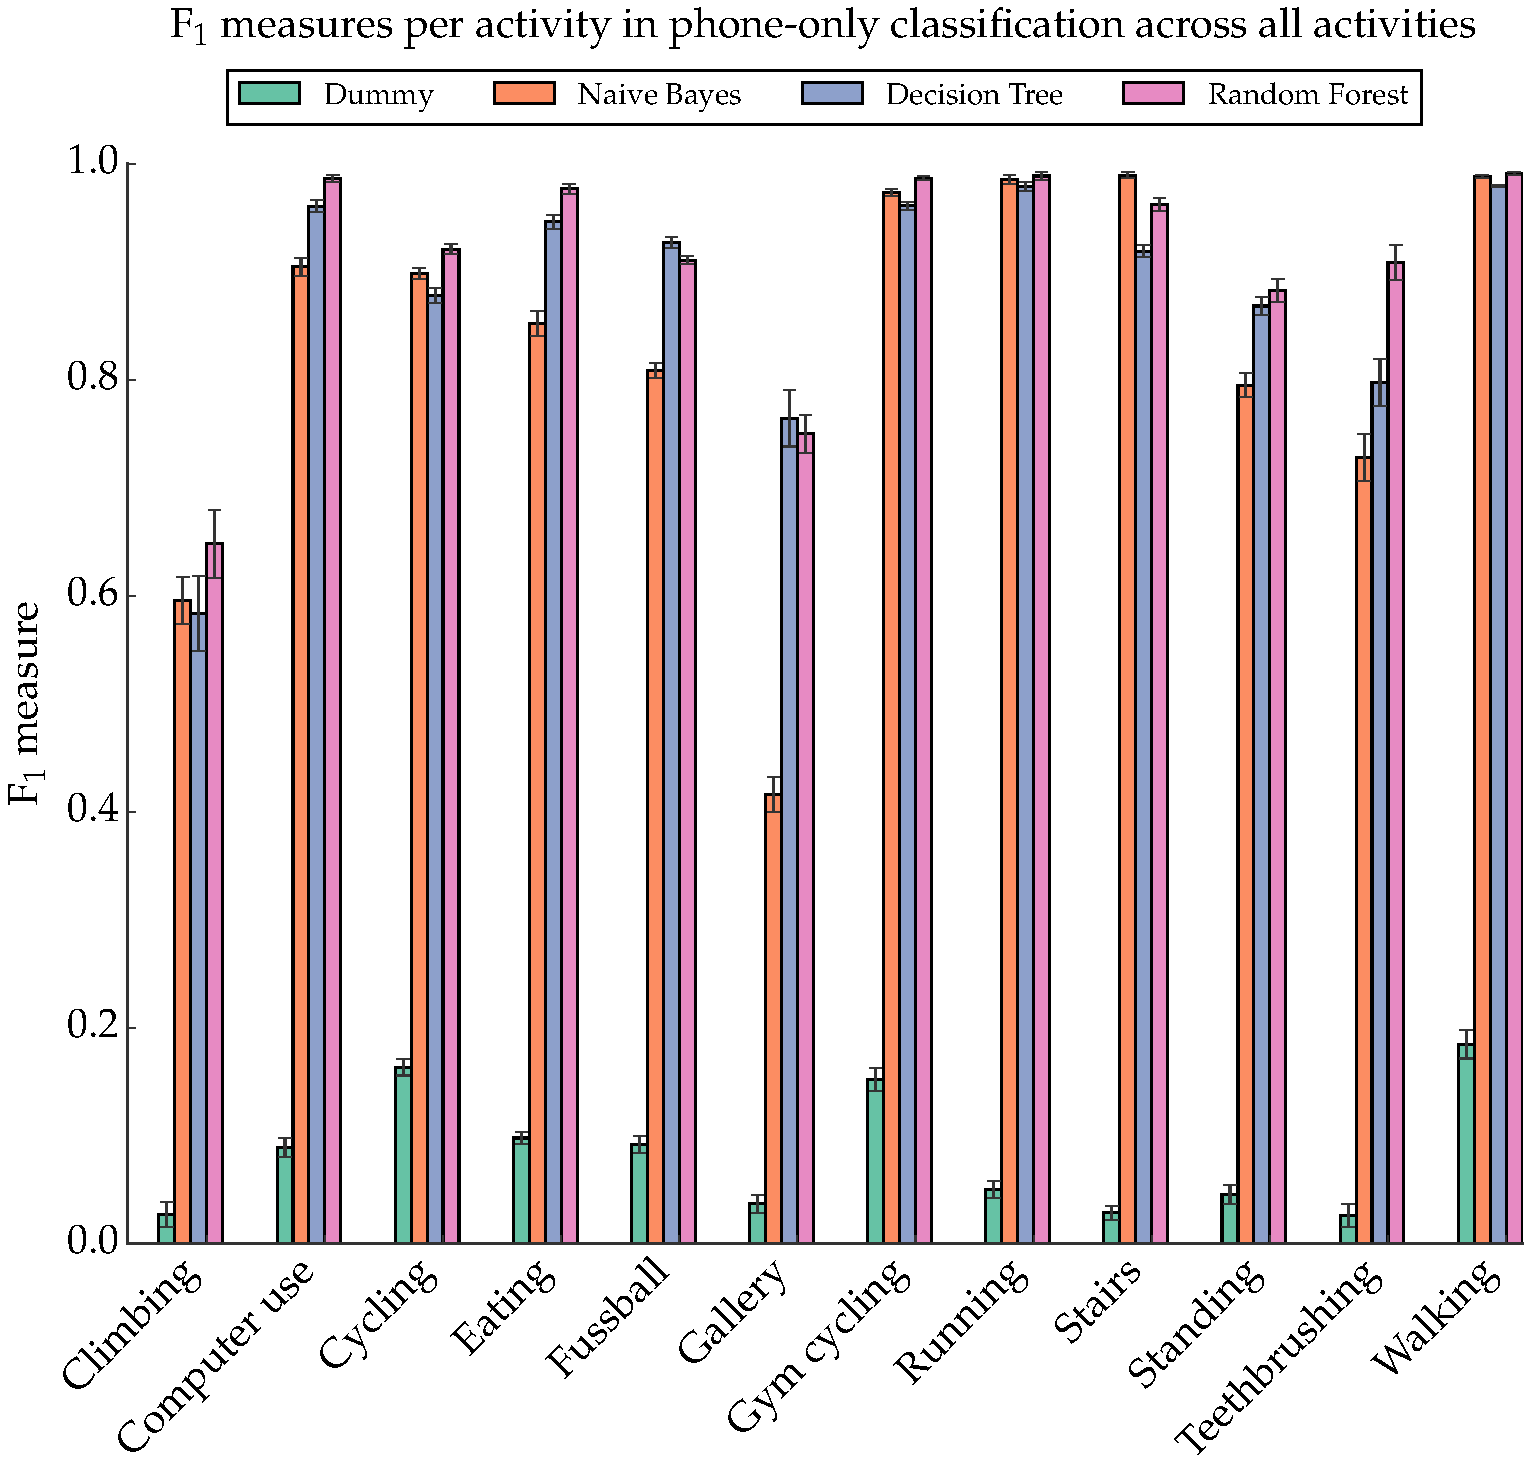
\includegraphics[width=1.0\textwidth]{F1GraphForEachClassifier_phone}
      \caption{$\mathrm{F}_1$ measures for each activity for each of the four classifiers trained on phone-only features.}
      \label{fig:F1GraphForEachClassifier_phone}
    \end{figure}
    
    Figure~\ref{fig:F1GraphAverage_phone} averages the $\mathrm{F}_1$ measures given in Figure~\ref{fig:F1GraphForEachClassifier_phone}. The random forest classifier outperforms the other three classifiers in average $\mathrm{F}_1$ measure. The decision tree and naive Bayes classifiers perform at the same level. Again, all three score significantly higher than the baseline dummy random classifier.
    
    \begin{figure}[htb]
      \centering
      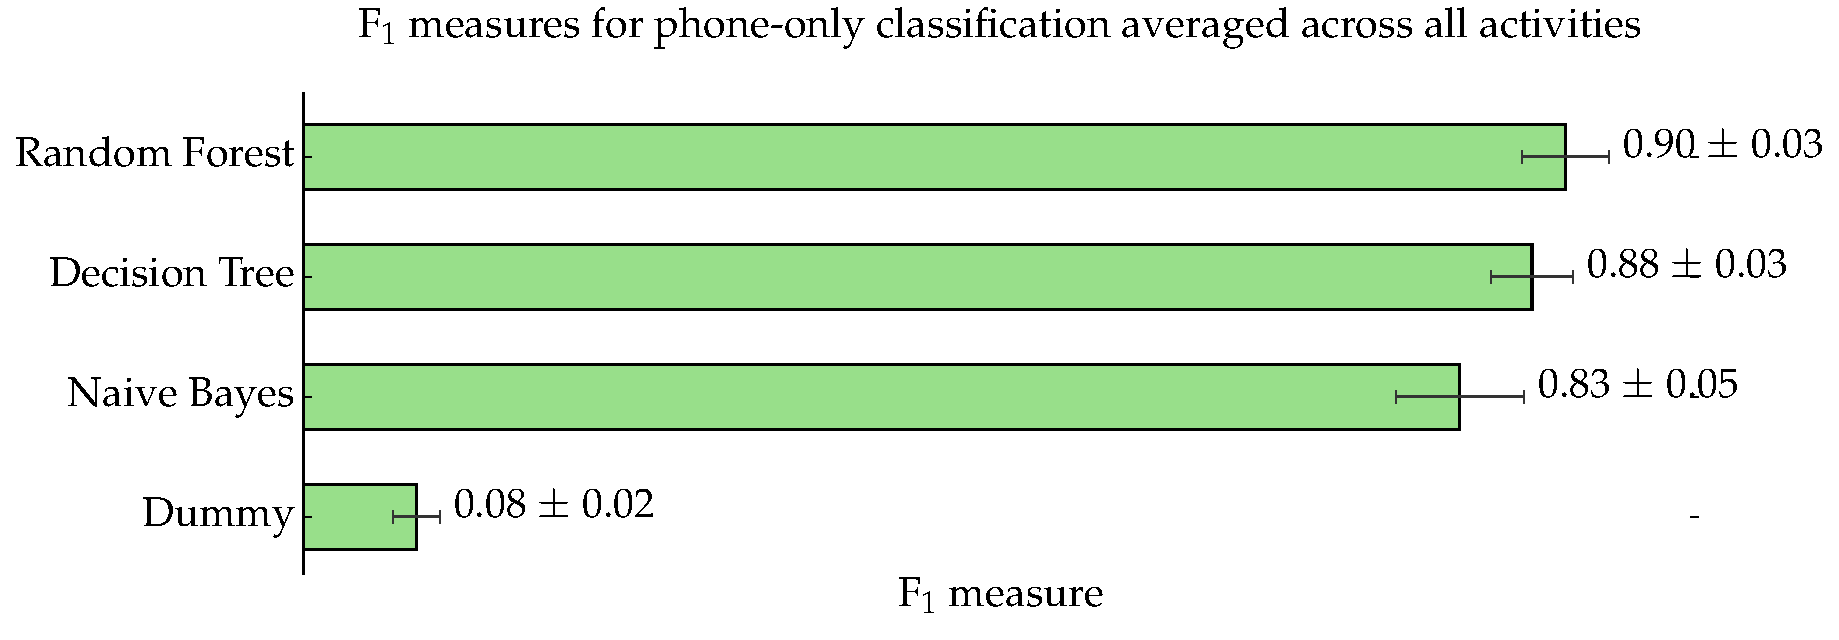
\includegraphics[width=1.0\textwidth]{F1GraphAverage_phone}
      \caption{Average $\mathrm{F}_1$ measures across all activities for each of the four classifiers trained on phone-only features. Error bars are calculated as the standard error in the mean. Best is 1, worst is 0.}
      \label{fig:F1GraphAverage_phone} 
    \end{figure}
    
    Table~\ref{tab:ConfusionMatrix_phone_RandomForestClassifier} presents a cumulative confusion matrix for the random forest classifier trained on phone-only features. The random forest classifier was chosen as the best performing classifier. The matrix is the addition of indvidiual confusion matrices from ten independent trials.
    
    From the confusion matrix, we see some of the misclassifications we would expect from phone-only classification:
    \begin{itemize}
      \item Computer use misclassified as eating, and vice versa. Both these activities are the only seated activities and the phone should struggle to differentiate between them.
      \item Gym cycling misclassified as cycling. Both of these activities exhibit the same pedalling motion in the leg, which phone data alone may struggle to differentiate.
      \item Many standing activities have been misclassified as each other, such as fussball, teethbrushing, standing and gallery perusal. Again, the phone data struggles to differentiate these static upright activities from each other.
    \end{itemize}  
    Note that the classifier has almost perfect precision on those activities that require highly periodic leg movements: gym cycling, running and walking. All (bar one) of the instances classified as those activities were correct.
    

    \begin{table}[htb]
      \tabcolsep=0.11cm
      \centering
        \begin{tabular}{lrrrrrrrrrrrr}
\toprule
Classified as $\rightarrow$ &    B &    U &     C &    E &    F &    G &     Y &    R &    S &    D &    T &     W \\
\midrule
B = Climbing      &  113 &    0 &    38 &    0 &   27 &    1 &     0 &    0 &    1 &    5 &    2 &     0 \\
U = Computer use  &    0 &  810 &     0 &   16 &    0 &    0 &     0 &    0 &    0 &    0 &    0 &     0 \\
C = Cycling       &   24 &    0 &  1336 &   11 &   25 &   10 &     1 &    0 &    3 &   16 &    4 &     0 \\
E = Eating        &    0 &    5 &     0 &  855 &    0 &    0 &     0 &    0 &    0 &    0 &    0 &     0 \\
F = Fussball      &   12 &    0 &    16 &    0 &  817 &   10 &     0 &    0 &    0 &    4 &    9 &     0 \\
G = Gallery       &    0 &    0 &     0 &    0 &   31 &  216 &     0 &    0 &    0 &   40 &    3 &     0 \\
Y = Gym cycling   &    0 &    0 &    37 &    0 &    0 &    0 &  1413 &    0 &    0 &    0 &    0 &     0 \\
R = Running       &    0 &    0 &     7 &    0 &    0 &    0 &     0 &  303 &    0 &    0 &    0 &     0 \\
S = Stairs        &    0 &    0 &    12 &    0 &    0 &    0 &     0 &    0 &  368 &    0 &    0 &     0 \\
D = Standing      &    0 &    0 &     0 &    0 &    6 &   22 &     0 &    0 &    0 &  432 &    0 &     0 \\
T = Teethbrushing &    0 &    0 &     1 &    9 &    6 &   13 &     0 &    0 &    0 &    0 &  220 &     0 \\
W = Walking       &    0 &    0 &    12 &    0 &    6 &    2 &     0 &    0 &    0 &    3 &    2 &  1745 \\
\bottomrule
\end{tabular}

      \caption{Cumulative confusion matrix from ten trials of the random forest classifier, the best performing of all the classifiers, trained on phone-only features.}
      \label{tab:ConfusionMatrix_phone_RandomForestClassifier}
    \end{table}
    
  \section{Watch-only measurements}
    The following results have been obtained by training each of the four classifiers on features extracted only from watch-collected accelerometer data.
    
    Figure~\ref{fig:F1GraphForEachClassifier_wear} gives the $\mathrm{F}_1$ measures for each activity resulting from classification using each of the four classifiers. Like in phone-only classification, the random forest classifier performs best of the four classifiers, outperforming others in 83\% of activities.
    
    Figure~\ref{fig:F1GraphAverage_wear} averages the $\mathrm{F}_1$ measures given in Figure~\ref{fig:F1GraphForEachClassifier_wear}. The random forest classifier outperforms the other three classifiers in average $\mathrm{F}_1$ measure. The decision tree performs marginally better than the naive Bayes classifier. Again, all three score significantly higher than the baseline dummy random classifier.
    
    Table~\ref{ConfusionMatrix_wear_RandomForestClassifier} presents a cumulative confusion matrix for the random forest classifier trained on watch-only features. Again, the random forest classifier was chosen as the best performing classifier. The matrix is the addition of indvidiual confusion matrices from ten independent trials.
    
    Compared to phone-only classification, the watch-only classifications exhibit less precision in those leg-period activities, such as running and walking. However, some periodicity is still present in the wrist movement and these activities are still classified accurately. A more interesting case is that of gym cycling, which is highly periodic in the leg movement but completely aperiodic in its wrist movement. As a result, its misclassification rate suffers.
    
    Standing activities also suffer from higher misclassification when using watch-only features.
    
    Unexpectedly, computer use and eating also are subject to a higher rate of misclassification than when using the phone-only features. Fussball, however, is better classified using the watch as opposed to the phone.
    \begin{figure}
      \centering
      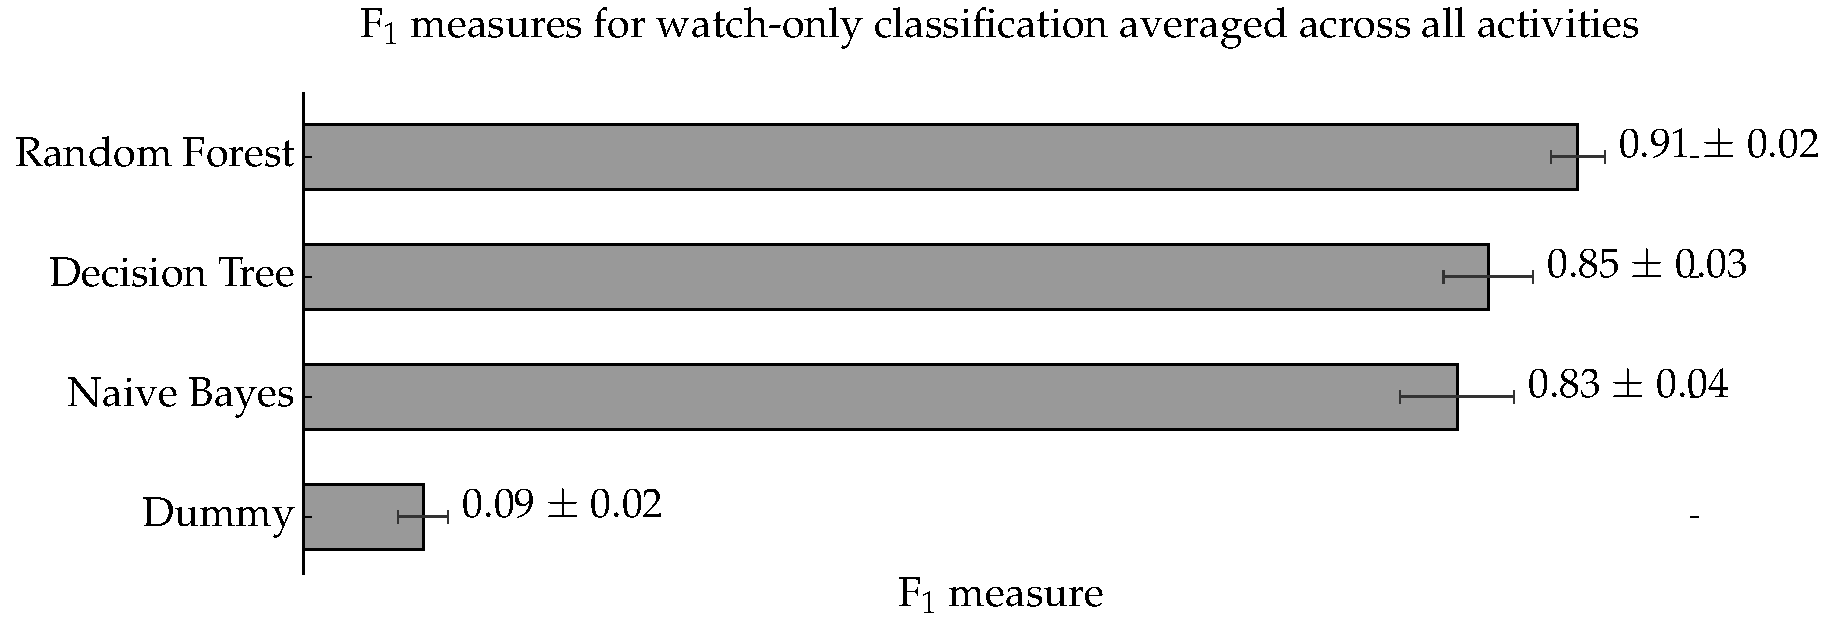
\includegraphics[width=1.0\textwidth]{F1GraphAverage_wear}
      \caption{Average $\mathrm{F}_1$ measures across all activities for each of the four classifiers trained on watch-only features. Error bars are calculated as the standard error in the mean. Best is 1, worst is 0. The random forest classifier again performs best overall.}
      \label{fig:F1GraphAverage_wear}
    \end{figure}

    \begin{figure}
      \centering
      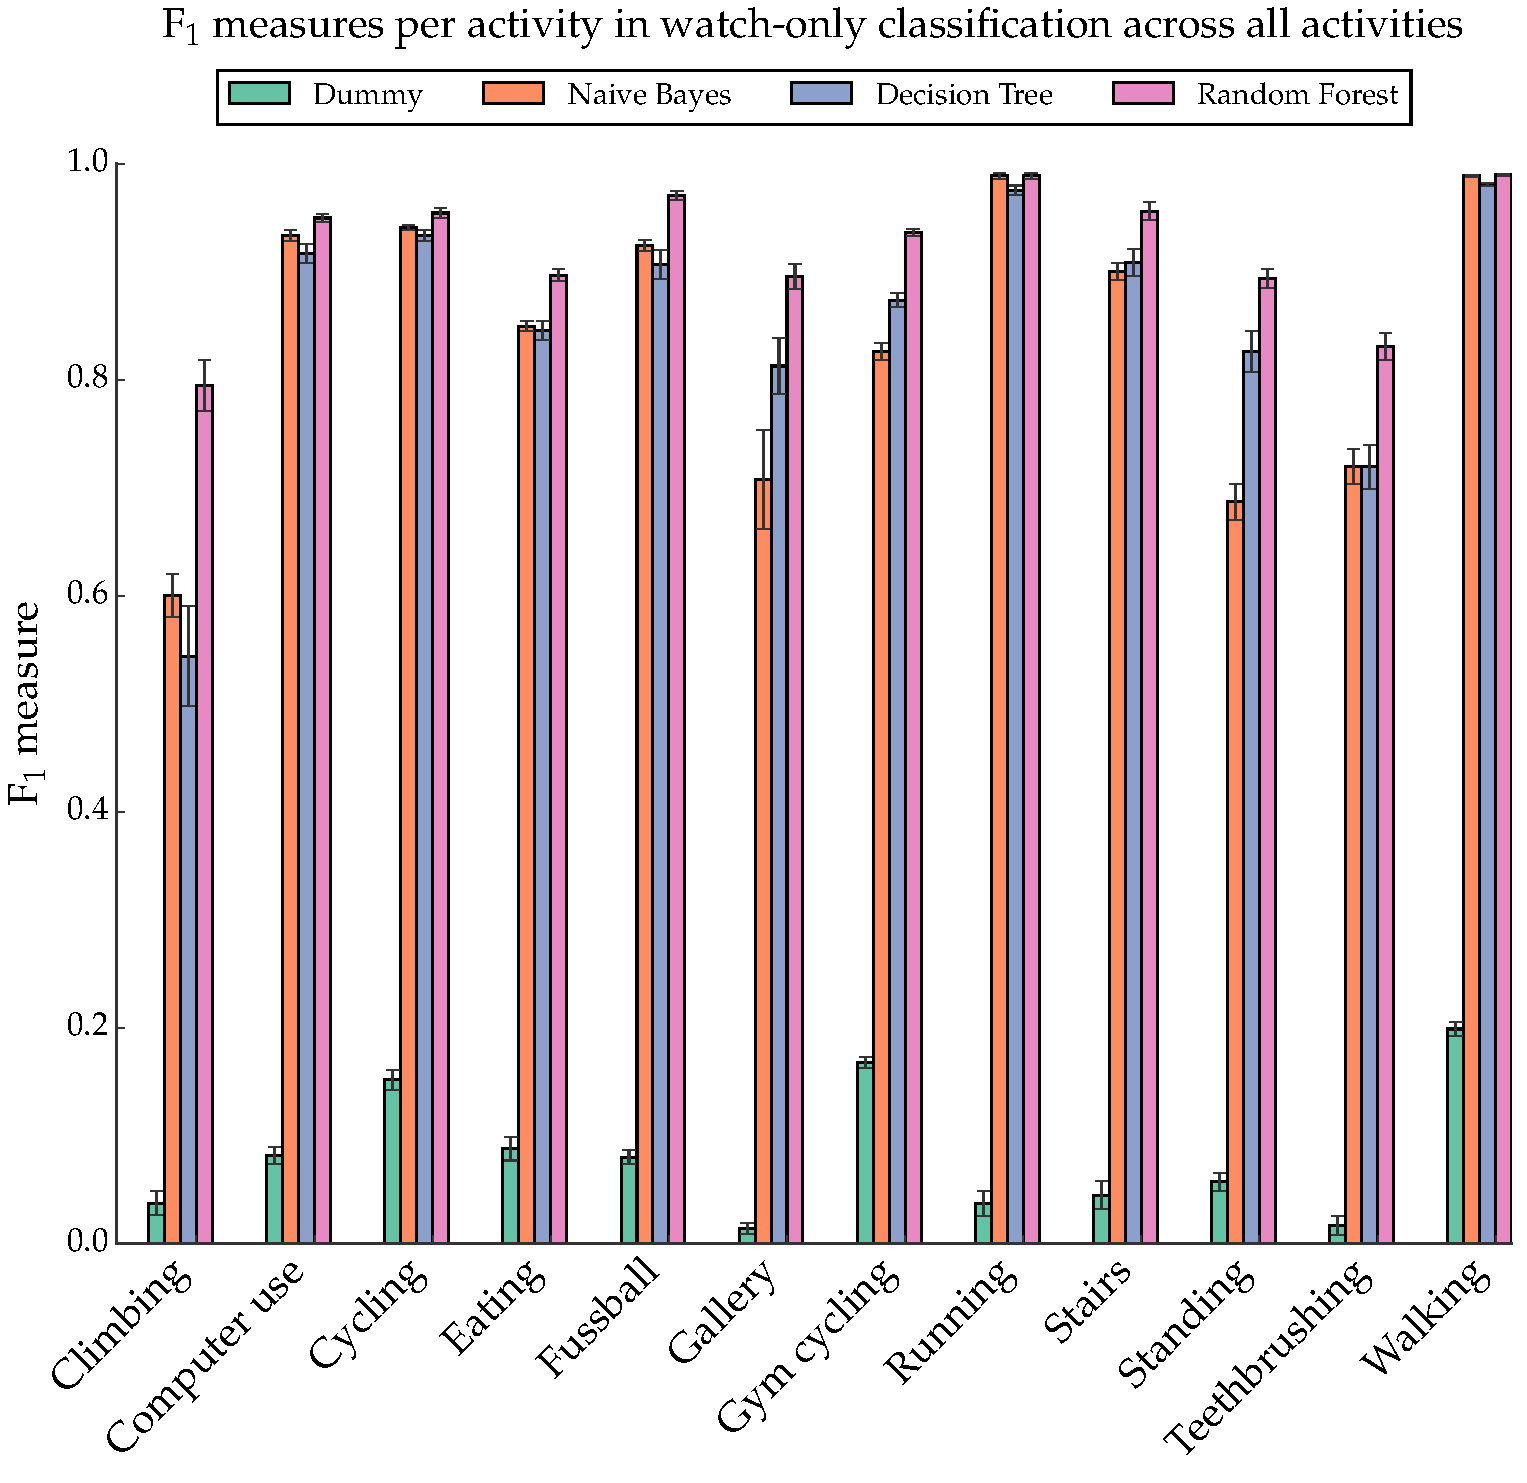
\includegraphics[width=1.0\textwidth]{F1GraphForEachClassifier_wear}
      \caption{$\mathrm{F}_1$ measures for each activity for each of the four classifiers trained on watch-only features.}
      \label{fig:F1GraphForEachClassifier_wear}
    \end{figure}
    
    \begin{table}
      \tabcolsep=0.11cm
      \centering
        \begin{tabular}{lrrrrrrrrrrrr}
\toprule
Classified as $\rightarrow$ &    B &    U &     C &    E &    F &    G &     Y &    R &    S &    D &    T &     W \\
\midrule
B = Climbing      &  133 &    0 &     6 &    3 &    0 &    4 &    36 &    0 &    8 &    0 &    0 &     0 \\
U = Computer use  &    0 &  767 &     0 &   39 &    0 &    0 &    15 &    0 &    0 &    5 &    0 &     0 \\
C = Cycling       &    3 &    0 &  1376 &    0 &   12 &   13 &     0 &    0 &    4 &   22 &    0 &     0 \\
E = Eating        &    1 &   19 &     0 &  812 &    0 &    0 &    25 &    0 &    0 &    3 &    0 &     0 \\
F = Fussball      &    0 &    0 &     7 &    1 &  851 &    3 &     4 &    0 &    3 &    0 &    0 &     1 \\
G = Gallery       &    0 &    0 &    19 &    0 &    0 &  261 &     0 &    0 &    0 &    5 &    4 &     1 \\
Y = Gym cycling   &    7 &   11 &     2 &   66 &    6 &    0 &  1352 &    0 &    3 &    3 &    0 &     0 \\
R = Running       &    0 &    0 &     2 &    0 &    0 &    0 &     0 &  304 &    0 &    0 &    0 &     4 \\
S = Stairs        &    0 &    0 &     0 &    5 &    0 &    0 &     1 &    0 &  374 &    0 &    0 &     0 \\
D = Standing      &    0 &    0 &    12 &    0 &    1 &   12 &    17 &    0 &    0 &  417 &    1 &     0 \\
T = Teethbrushing &    0 &    0 &    12 &   14 &    4 &    9 &     6 &    0 &    0 &    3 &  196 &     0 \\
W = Walking       &    1 &    0 &     9 &    1 &    1 &    0 &     1 &    0 &    9 &    0 &    0 &  1748 \\
\bottomrule
\end{tabular}

      \caption{Cumulative confusion matrix from ten trials of the random forest classifier, the best performing of all the classifiers, trained on watch-only features.}
      \label{tab:ConfusionMatrix_wear_RandomForestClassifier}
    \end{table}
    
  
  \section{Phone and watch measurements}
    The following results have been obtained by training each of the four classifiers on features extracted from both phone and watch accelerometer data.
    
    Figure~\ref{fig:F1GraphForEachClassifier_both} gives the $\mathrm{F}_1$ measures for each activity resulting from classification using each of the four classifiers trained on phone and watch features. Like in phone-only and watch-only classification, the random forest classifier performs best of the four classifiers, outperforming others in 67\% of activities. This percentage however is the lowest of the three feature-set cases. The naive Bayes classifier performs better in more types of activities than the decision tree classifier. This is particularly evident in those activities identified to be  periodic: cycling, gym cycling, running, stairs, teethbrushing and walking.
    
    Figure~\ref{fig:F1GraphAverage_both} averages the $\mathrm{F}_1$ measures given in Figure~\ref{fig:F1GraphForEachClassifier_both}. The random forest classifier outperforms the other three classifiers in average $\mathrm{F}_1$ measure. The decision tree and naive Bayes classifiers both score equally at the $\mathrm{F}_1$ measure. Again, all three score significantly higher than the baseline dummy random classifier.
    
    Table~\ref{tab:ConfusionMatrix_both_RandomForestClassifier} presents a cumulative confusion matrix for the random forest classifier trained on both phone and watch features. Again, the random forest classifier was chosen as the best performing classifier.
    
    Using both phone and watch features reduces the effect of the broad categories of uncertainty that were present in phone-only and watch-only classification, though in many cases the difference is negliable. The only activity in which using phone and watch features together significantly outperforms either phone or watch classification on its own is in the climbing activitiy.
    
    \begin{figure}
      \centering
      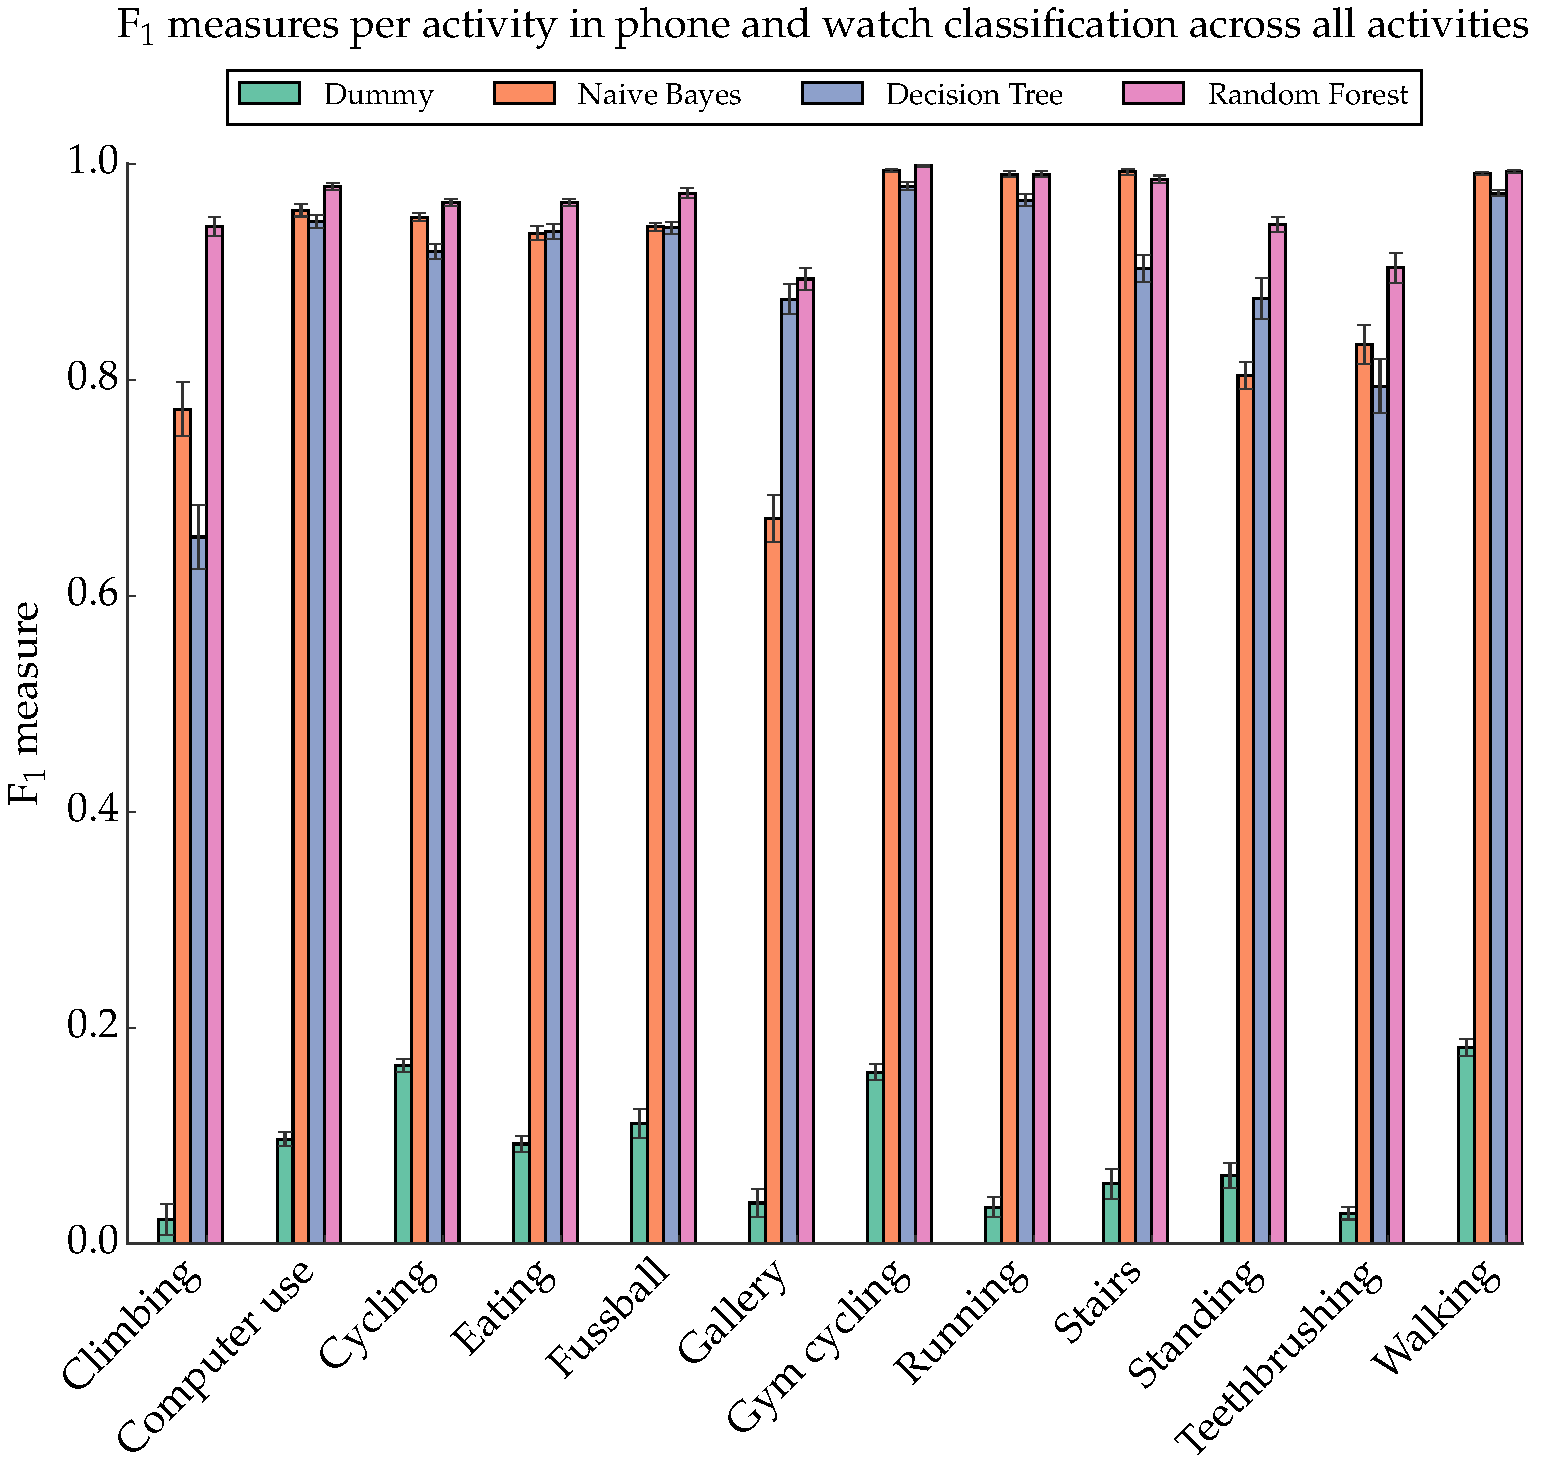
\includegraphics[width=1.0\textwidth]{F1GraphForEachClassifier_both}
      \caption{$\mathrm{F}_1$ measures for each activity for each of the four classifiers trained on both phone and watch features.}
      \label{fig:F1GraphForEachClassifier_both}
    \end{figure}
    
    \begin{figure}
      \centering
      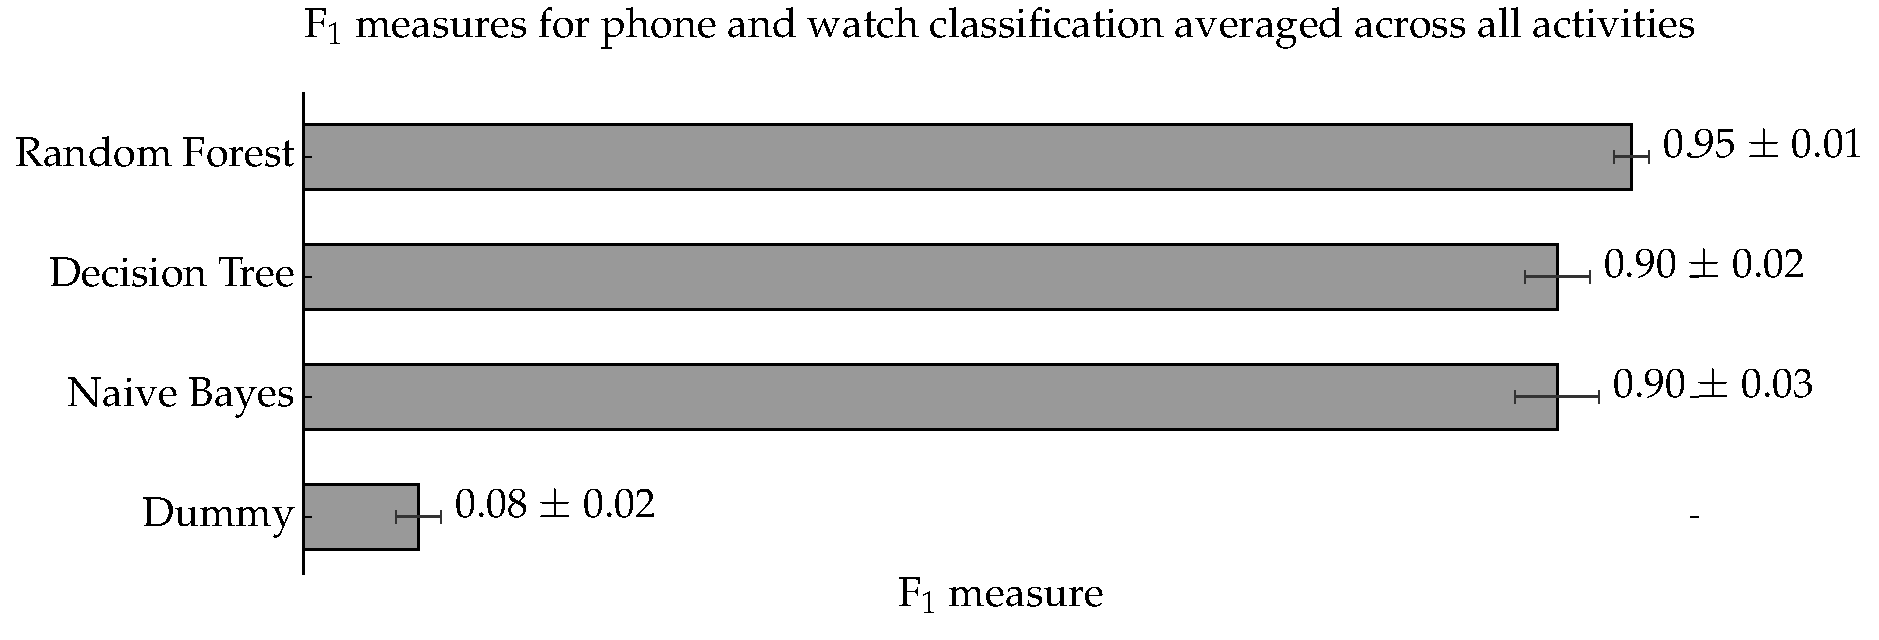
\includegraphics[width=1.0\textwidth]{F1GraphAverage_both}
      \caption{Average $\mathrm{F}_1$ measures across all activities for each of the four classifiers trained on both phone and watch features. Error bars are calculated as the standard error in the mean. Best is 1, worst is 0.}
      \label{fig:F1GraphAverage_both}
    \end{figure}
    
    \begin{table}
      \tabcolsep=0.11cm
      \centering
        \begin{tabular}{lrrrrrrrrrrrr}
\toprule
Classified as $\rightarrow$ &    B &    U &    C &    E &    F &    G &    Y &    R &    S &    D &    T &    W \\
\midrule
B = Climbing      & 0.89 & 0.01 & 0.03 & 0.02 & 0.02 & 0.02 &  0 &  0 & 0.01 & 0.01 & 0.01 &  0 \\
U = Computer use  &  0 & 0.96 &  0 & 0.04 &  0 &  0 &  0 &  0 &  0 &  0 &  0 &  0 \\
C = Cycling       &  0 &  0 & 0.97 & 0.00 & 0.01 & 0.01 &  0 &  0 &  0 & 0.01 & 0.00 &  0 \\
E = Eating        &  0 & 0.01 &  0 & 0.99 &  0 &  0 &  0 &  0 &  0 &  0 &  0 &  0 \\
F = Fussball      &  0 &  0 & 0.01 &  0 & 0.99 &  0 &  0 &  0 &  0 &  0 &  0 &  0 \\
G = Gallery       &  0 &  0 & 0.00 &  0 & 0.02 & 0.92 &  0 &  0 &  0 & 0.05 &  0 &  0 \\
Y = Gym cycling   & 0.01 &  0 &  0 &  0 &  0 &  0 & 0.99 &  0 &  0 &  0 &  0 &  0 \\
R = Running       &  0 &  0 & 0.01 &  0 &  0 &  0 &  0 & 0.97 & 0.00 &  0 &  0 & 0.01 \\
S = Stairs        &  0 &  0 & 0.02 &  0 &  0 &  0 &  0 &  0 & 0.98 &  0 &  0 &  0 \\
D = Standing      &  0 &  0 & 0.00 & 0.00 & 0.02 & 0.04 &  0 &  0 &  0 & 0.93 & 0.01 &  0 \\
T = Teethbrushing & 0.00 &  0 & 0.04 & 0.07 & 0.00 & 0.04 &  0 &  0 &  0 & 0.02 & 0.83 &  0 \\
W = Walking       &  0 &  0 & 0.01 &  0 & 0.00 & 0.00 &  0 &  0 & 0.00 & 0.00 & 0.00 & 0.99 \\
\bottomrule
\end{tabular}

      \caption{Cumulative confusion matrix from ten trials of the random forest classifier, the best performing of all the classifiers, trained on both phone and watch features.}
      \label{tab:ConfusionMatrix_both_RandomForestClassifier}
    \end{table}
  
  \section{Comparison}
    This section presents graphs that directly compare the $\mathrm{F}_1$ measures as calculated by classifiers trained with phone-only, watch-only and phone and watch feature sets.
    
    Figure~\ref{fig:F1Graph_RandomForestClassifier} gives {$\mathrm{F}_1$ measures for each activity using the random forest classifier trained on each of the three feature sets. On average, the random forest classifier performed best and so is discussed primarily in this evaluation.
    
    Climbing is the only activity in which using both phone and watch feature sets significantly outperforms either feature set on its own. In all other trials, using both the phone and watch feature sets was better but not significantly so. This is not necessarily because using both feature sets performed badly, but because both the phone-only and watch-only feature sets performed well. 
  
    Figure~\ref{fig:F1Graph_average_f1_per_featureset} averages {$\mathrm{F}_1$ measures across all activities grouped by classifier and feature set. In all three of the classifers, the phone and watch outperform phone-only features and watch-only features. On average, the phone-only and the watch-only features perform equally well.
    
    A particularly interesting result is that phone-only classification performs best in computer use and eating classification; introducing features extracted from watch data actually reduces the accuracy of the classifier. It is paradoxical that adding more data would make classification less accurate, especially as most of the information to be gained from computer use and eating activities should come from the watch rather than the phone.
    
    One possible reason for this misclassification is the lack of other seated activities. Computer use and eating are the only two seated acitivities. Contrast this to semi-stationary standing activities such as fussball, standing, gallery perusal or teethbrushing. Watch-only classification consistently outperforms phone-only classification in these activities, while phone-only classification scores lower in each case than it does for computer use or for eating. I'd argue that one's ability to classify a certain activity depends very much on the other activities present in the dataset and how fine the nuances are between them. 
    
        The second of the two overall aims of the project was to evaluate to what extent the smartwatch is better at helping to classify activities. Both figures here show the the smartwatch is just as good as the smartphone, outperforming just the smartwatch in some activities and performing marginally better on average, though it is not statistically significant. Using both phone and watch features outperforms both on average and on a per-device level.
    \begin{figure}
      \centering
      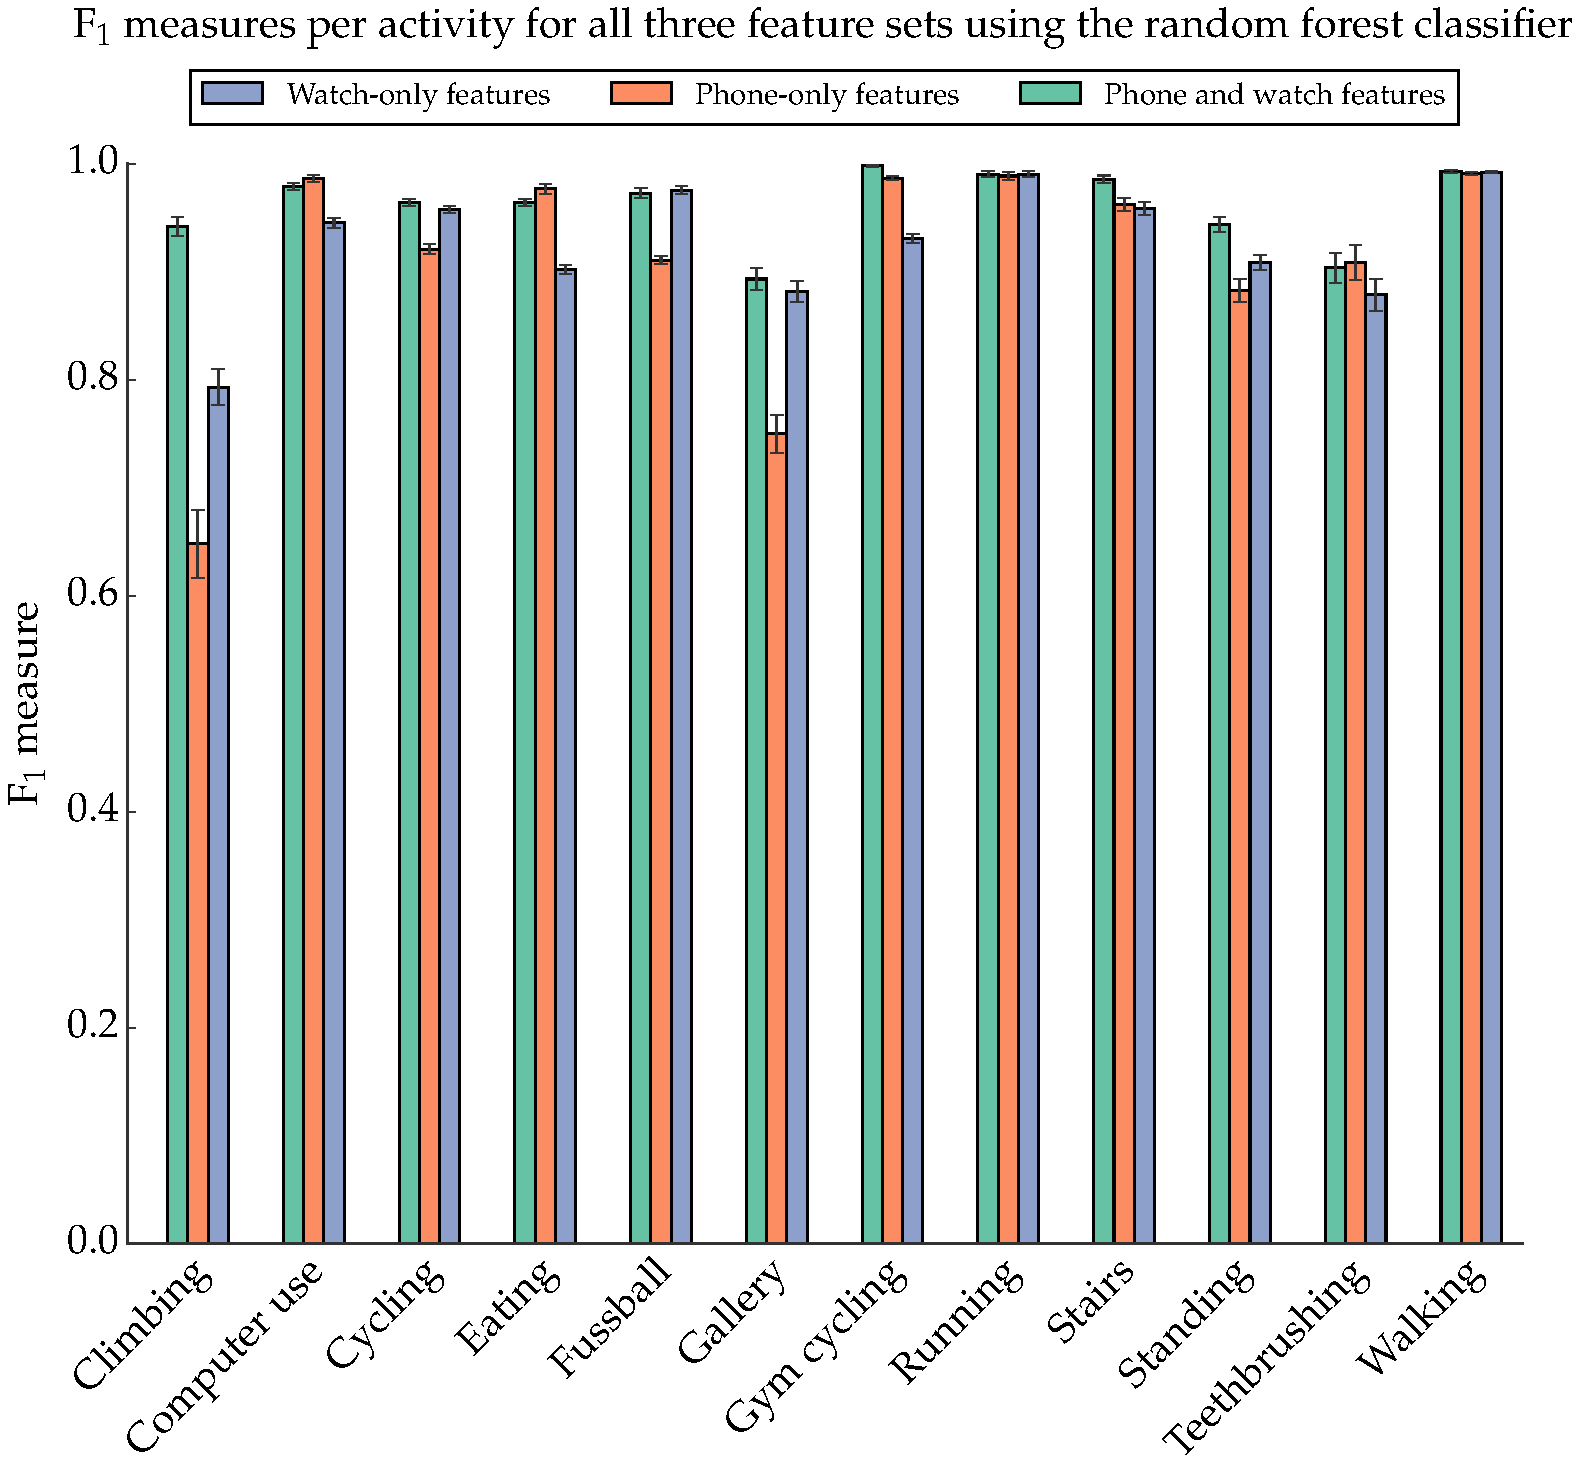
\includegraphics[width=1.0\textwidth]{F1Graph_RandomForestClassifier}
      \caption{$\mathrm{F}_1$ measures for each activity using the random forest classifier trained on phone-only, wear-only and both phone and wear features.}
      \label{fig:F1Graph_RandomForestClassifier}
    \end{figure}
    \begin{figure}
      \centering
      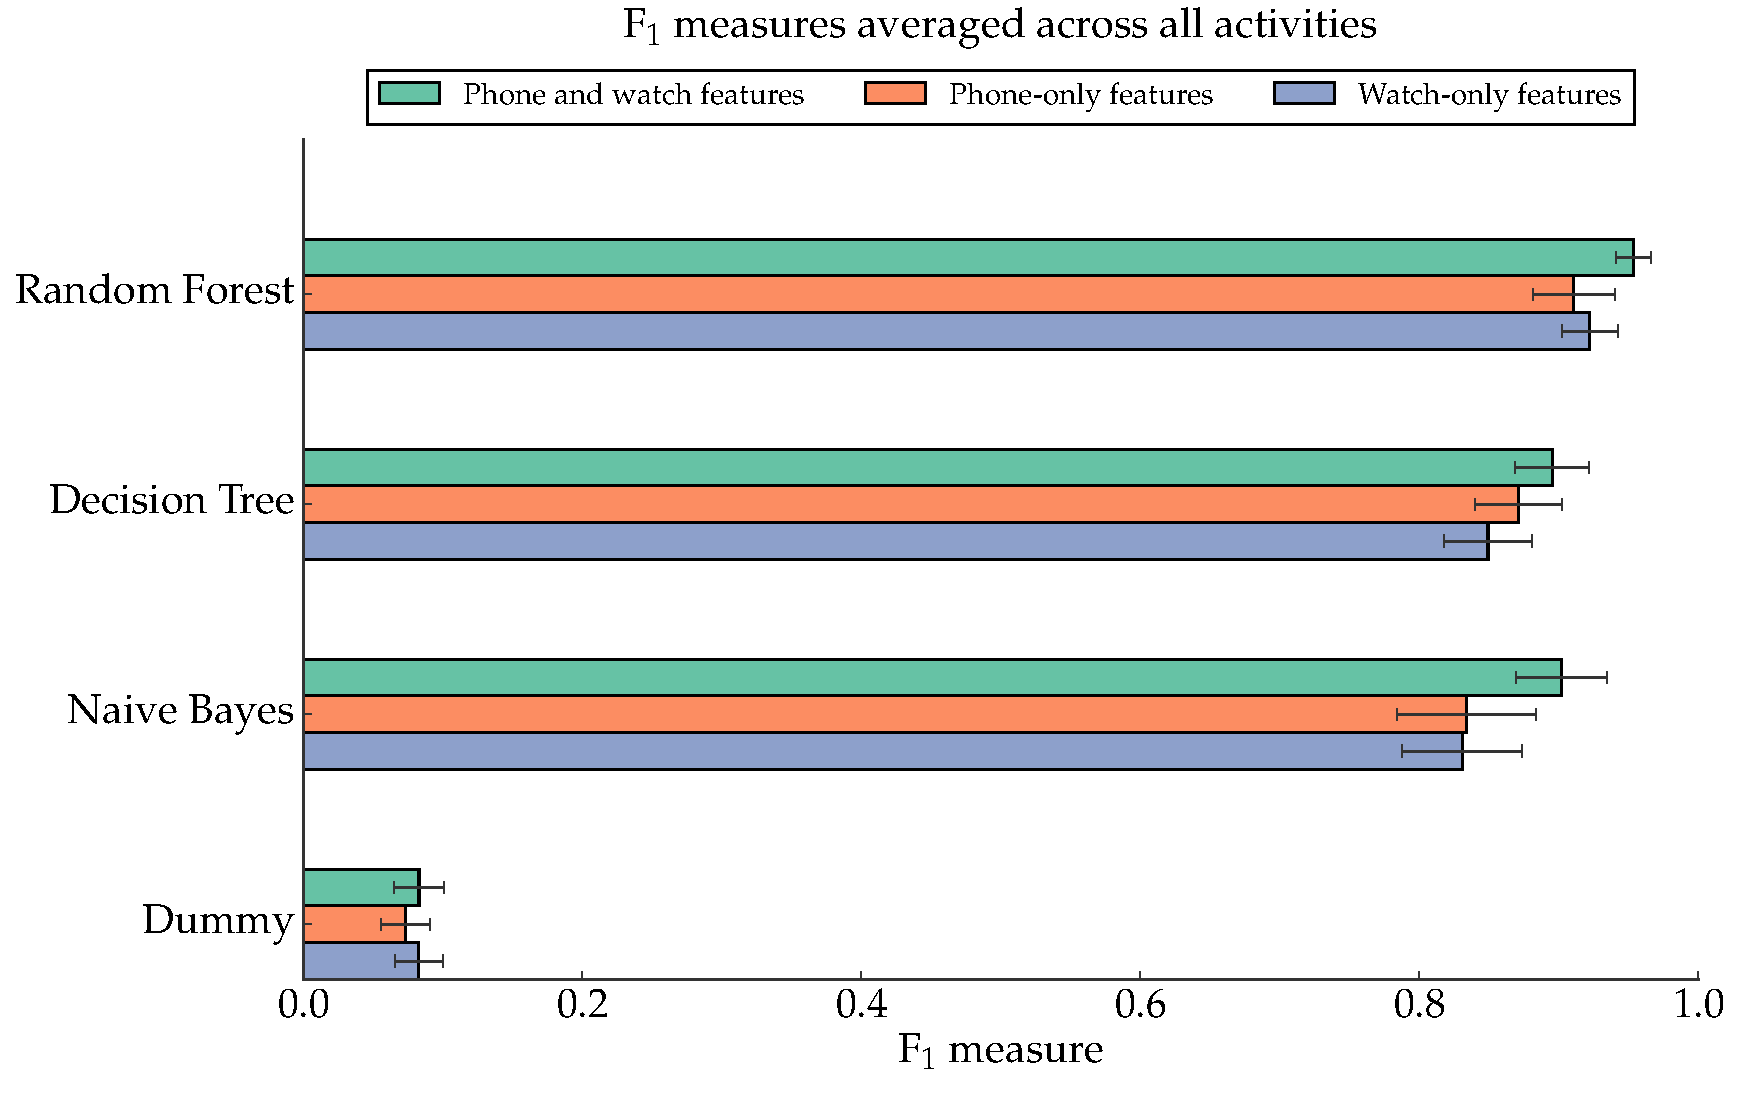
\includegraphics[width=1.0\textwidth]{F1Graph_average_f1_per_featureset}
      \caption{Average $\mathrm{F}_1$ measures for each activity from all classifiers, trained on phone-only, wear-only and both phone and wear features.}
      \label{fig:F1Graph_average_f1_per_featureset}
    \end{figure}
  
  \section{Feature importances}
    Feature importances can be calculated when using decision trees and random forests. Feature importances, also known as Gini importance, is the normalised total reduction in impurity brought by that feature\cite{breiman2001random}. A feature that can split the whole dataset into exactly two labels would have a feature importance of 1.
    
    In the case of classifcation using both phone and watch features, we would expect to see a mix of features from both devices.
    
    Figure~\ref{fig:FeatureImportancesTogether} presents the top five most important features from phone-only, watch-only and both phone and watch classification. The feature importances were averaged from 50 component decision trees of a random forest classifier. As expected, phone and watch features are equally important in the phone and watch classification task. 
    
    This method is also useful to evaluate feature selection. Of all features calculated, three general classes of feature stand out as being important:
    \begin{enumerate}
      \item correlation between axes;
      \item spectral flatness, a measure of periodicity; and
      \item peak frequency.
    \end{enumerate}
    These three classes of feature can be collected just as easily on the watch as on the phone, and the quality of data seems to be comparable.
    
    Figure~\ref{fig:FeatureImportancesCumulative} gives cumulative feature importances for each activity. A random forest classifier was given both phone and watch features but was trained using sets of one vs. rest binary labels. That is, for each activity $\chi$, the labels were converted into having two possible values: $\chi$ and $\bar{\chi}$. This allows extraction of feature importances per activity.
    
    Feature importances for some activities are understandable: phone features are more important when classifying stairs, standing and walking. Some, however, make less sense. As discussed earlier, computer use and eating also assign more importance to phone features, while cycling is the activity that assigns the most importance to watch features.
    
    One possible reason for this observation is that while phone features are good enough to place cycling into a general class of leg-periodic activities, differentiating them requires more information than is available through the phone alone. Though the most charactistic movements could come from one accelerometer, these could be shared with other activities. A second accelerometer that does not necessarily follow those characteristic movements, such as the watch while cycling, could potentially be used to nuance the results and differentiate cycling from, say, cycling in the gym.
    
    \begin{figure}
      \centering
      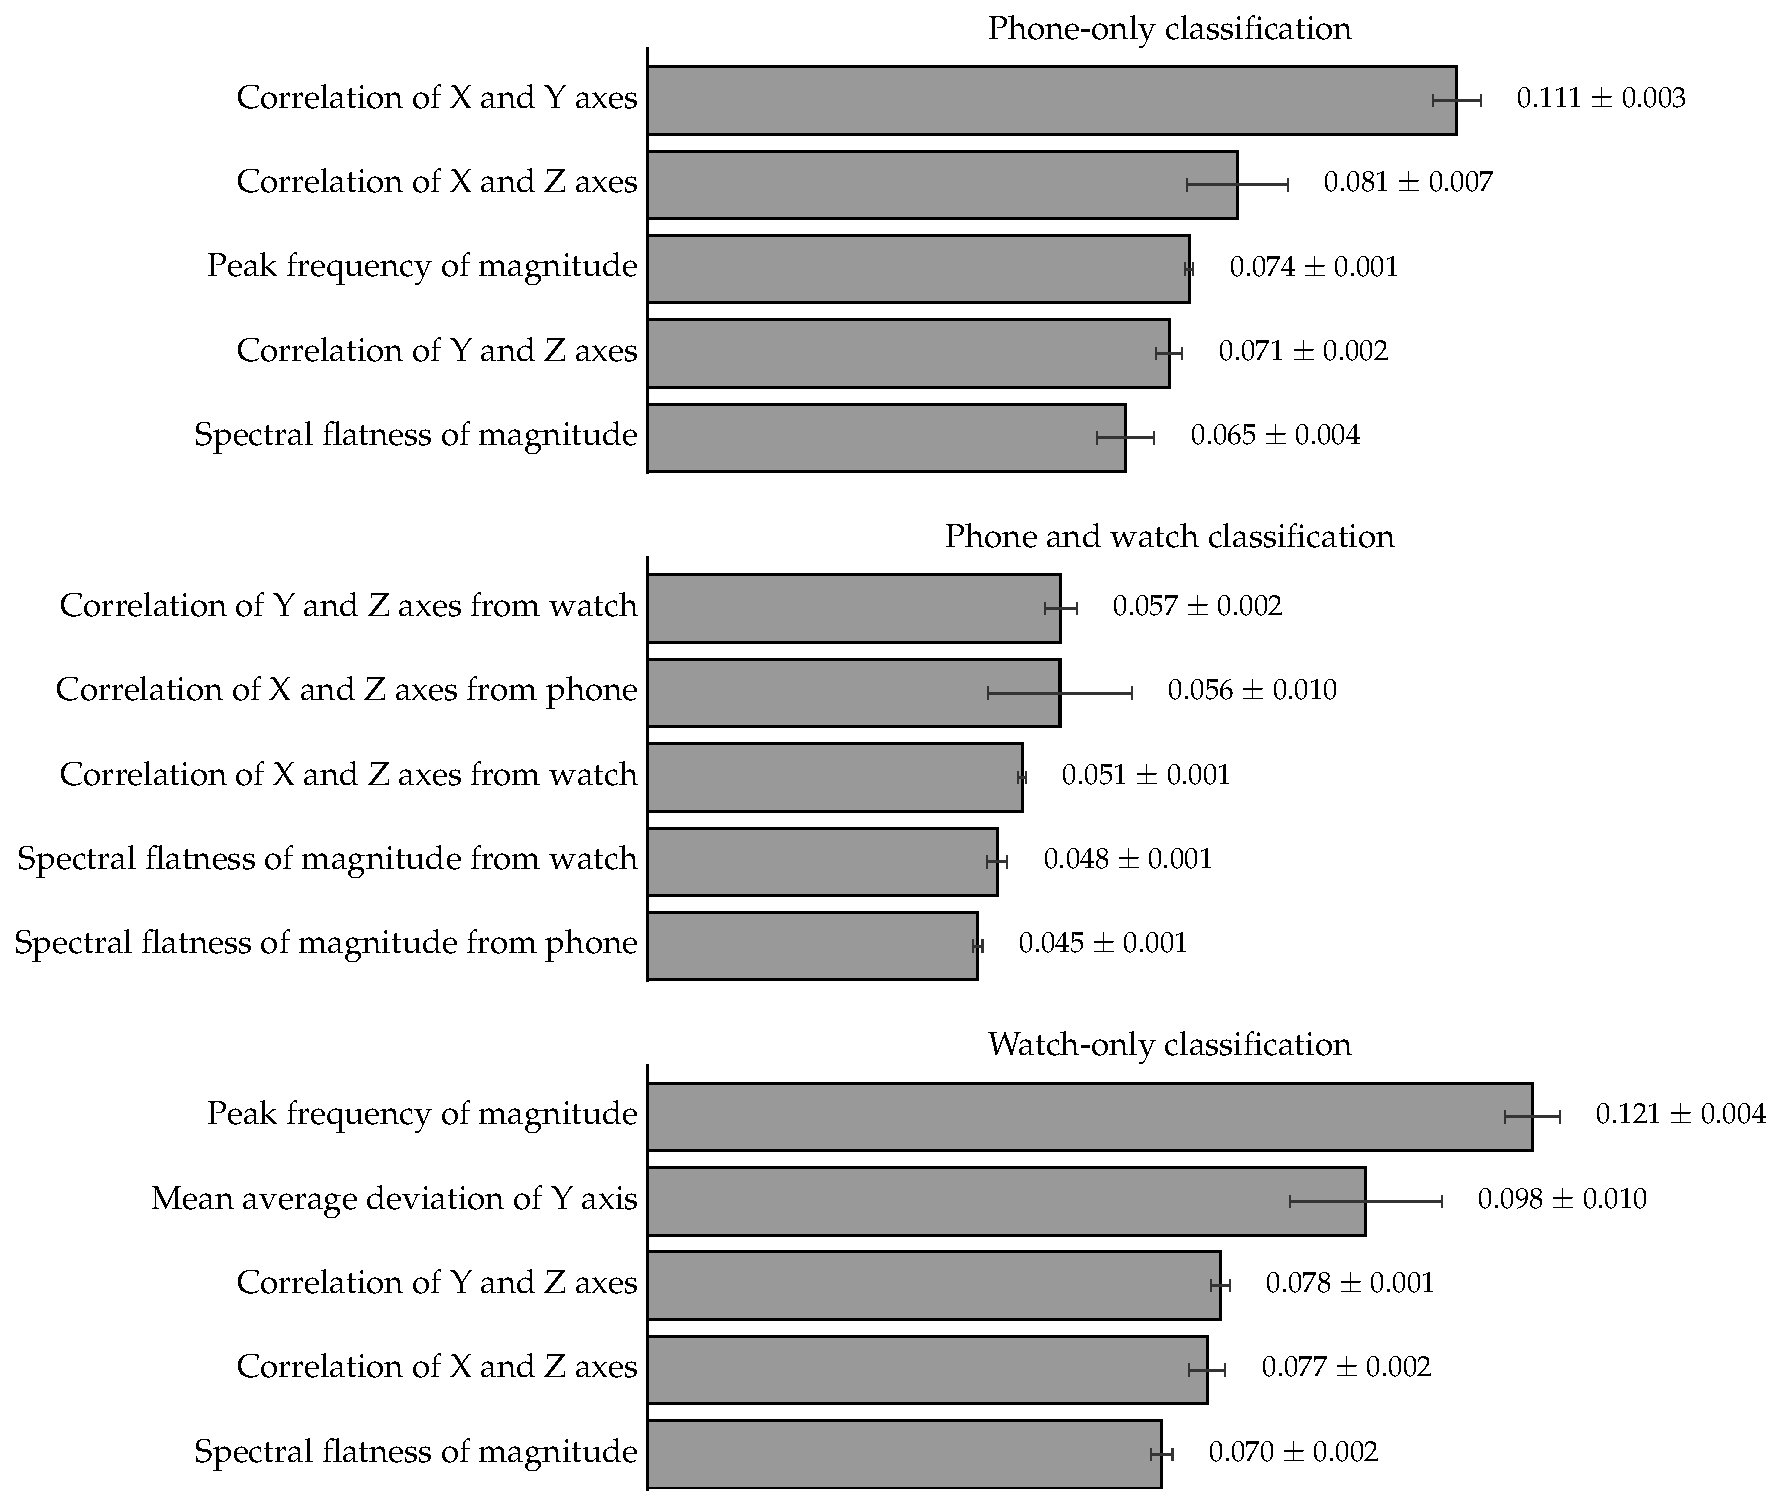
\includegraphics[width=1.0\textwidth]{FeatureImportancesTogether}
      \caption{Feature importances of the top five most important features averaged over 50 decision trees in a random forest classifier trained with the three feature sets. Recall that data from the phone and the watch each produce 22 features, and so phone and watch classification has 44 features from which to pick.}
      \label{fig:FeatureImportancesTogether}
    \end{figure}
    
    \begin{figure}
      \centering
      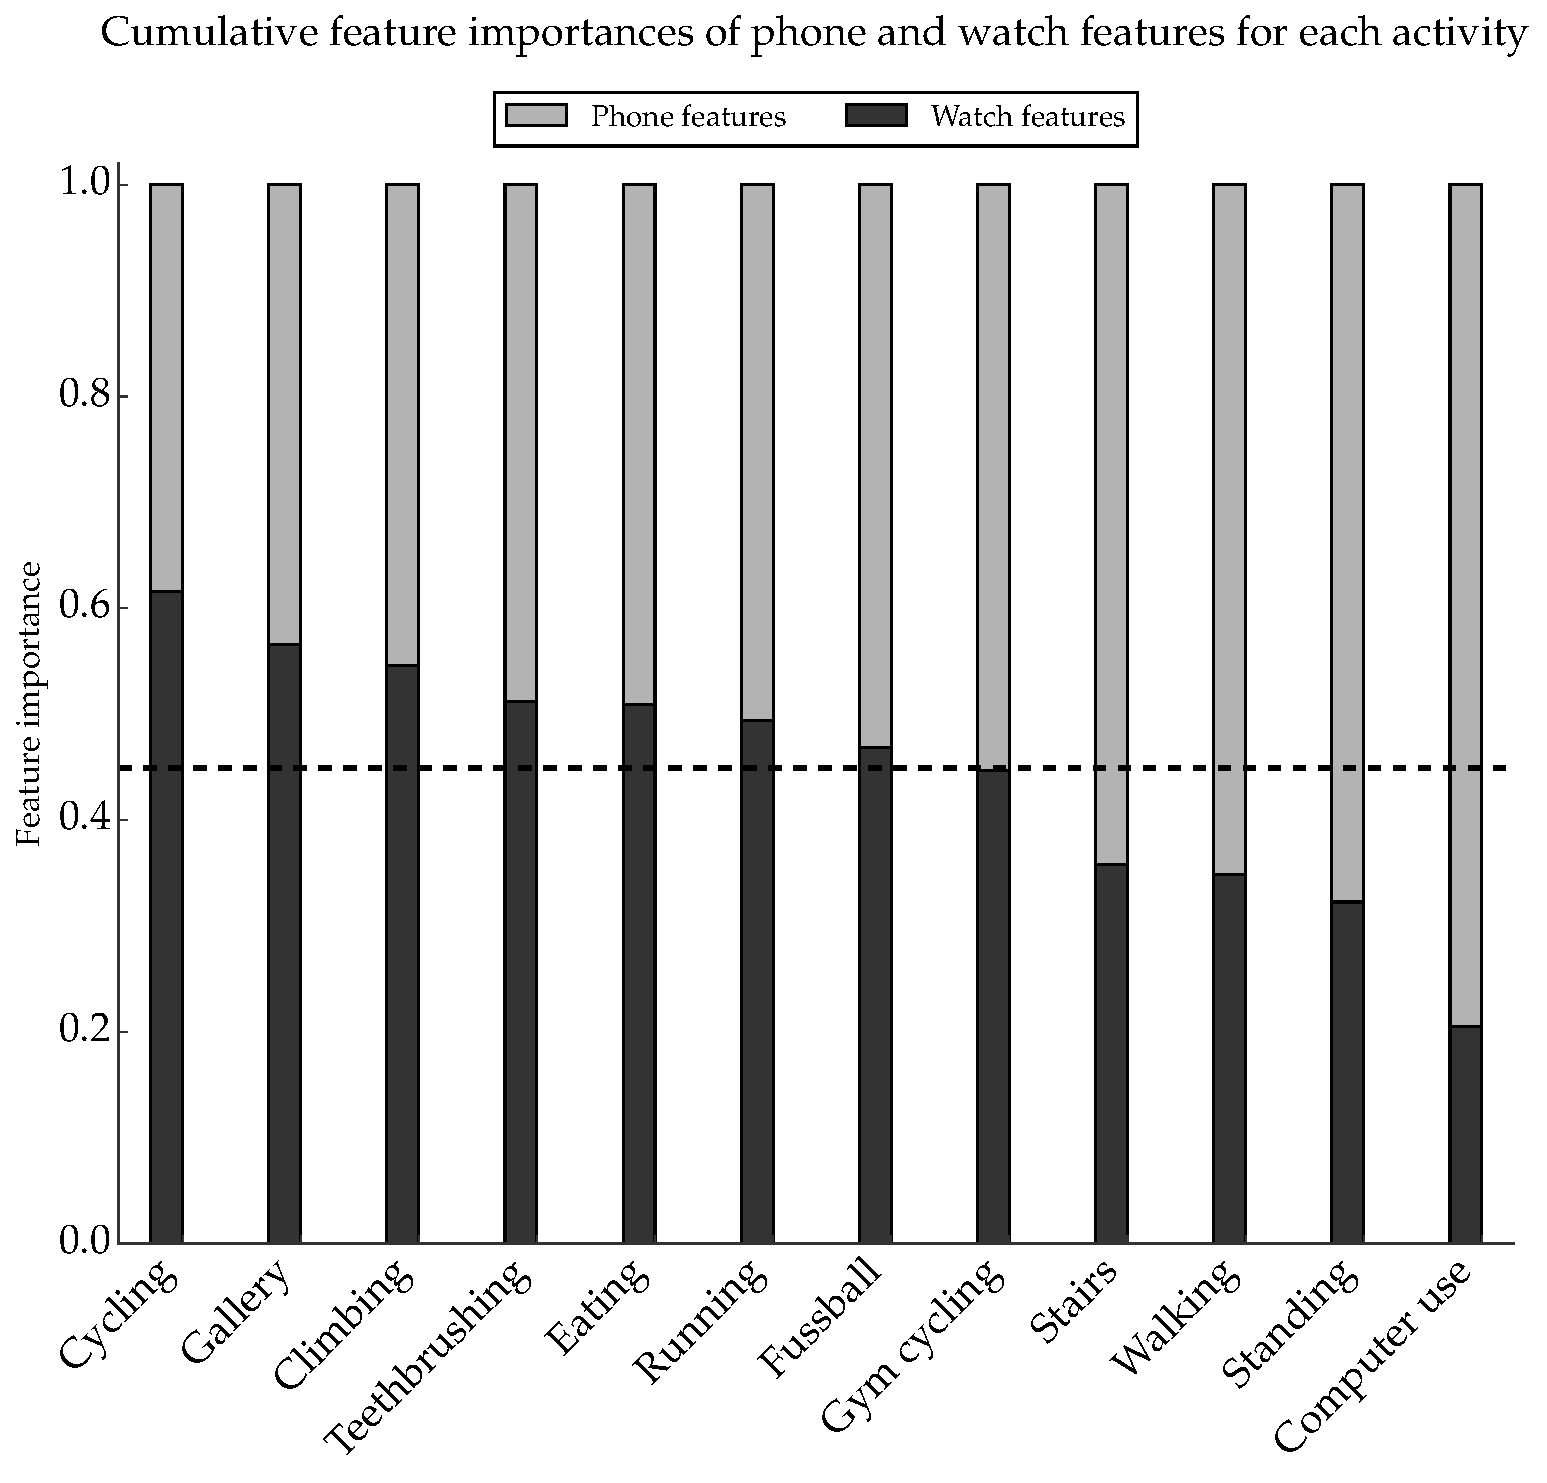
\includegraphics[width=1.0\textwidth]{FeatureImportancesCumulative}
      \caption{Cumulative feature importances for each activity. A random forest classifier was trained with one vs. rest labels and both phone and watch features. The importances of all the phone features and of all the watch features were totalled separately. The average total watch feature importance, $\approx 0.42$ is marked as the dotted line on the graph.}
      \label{fig:FeatureImportancesCumulative}
    \end{figure}
  \section{Summary}
    In this section I compare $\mathrm{F}_1$ measures per activity and on average over all activities between phone-only features, watch-only features and both phone and watch features classification. I also present confusion matrices for each of these three feature sets.
    
    In terms of $\mathrm{F}_1$ measure, phone and watch classification outperforms either device individually. Watch classification marginally outperforms phone classification. The range of $\mathrm{F}_1$ measures between the three sets of classification is not large, but this is primarily because there is not much scope to improve on using either device individually: they both individualy score >0.9 on the $\mathrm{F}_1$ measure on average across all activities.
    
    I also use feature importance from decision trees to evaluate phone and watch features. This method calculates that watch features have an average total importance of 0.42 compared to the phone's 0.58. Some activities a total importance as high as 0.6 to watch features, while others are as low as 0.2.